
\section{Communication and Data Integration}

\subsection{MQTT Protocol}
The MQTT protocol was chosen for its lightweight communication capabilities, particularly suitable for Industrial IoT environments. This enabled real-time updates between the lab equipment and the central system.
\begin{figure}[H]
    \centering
    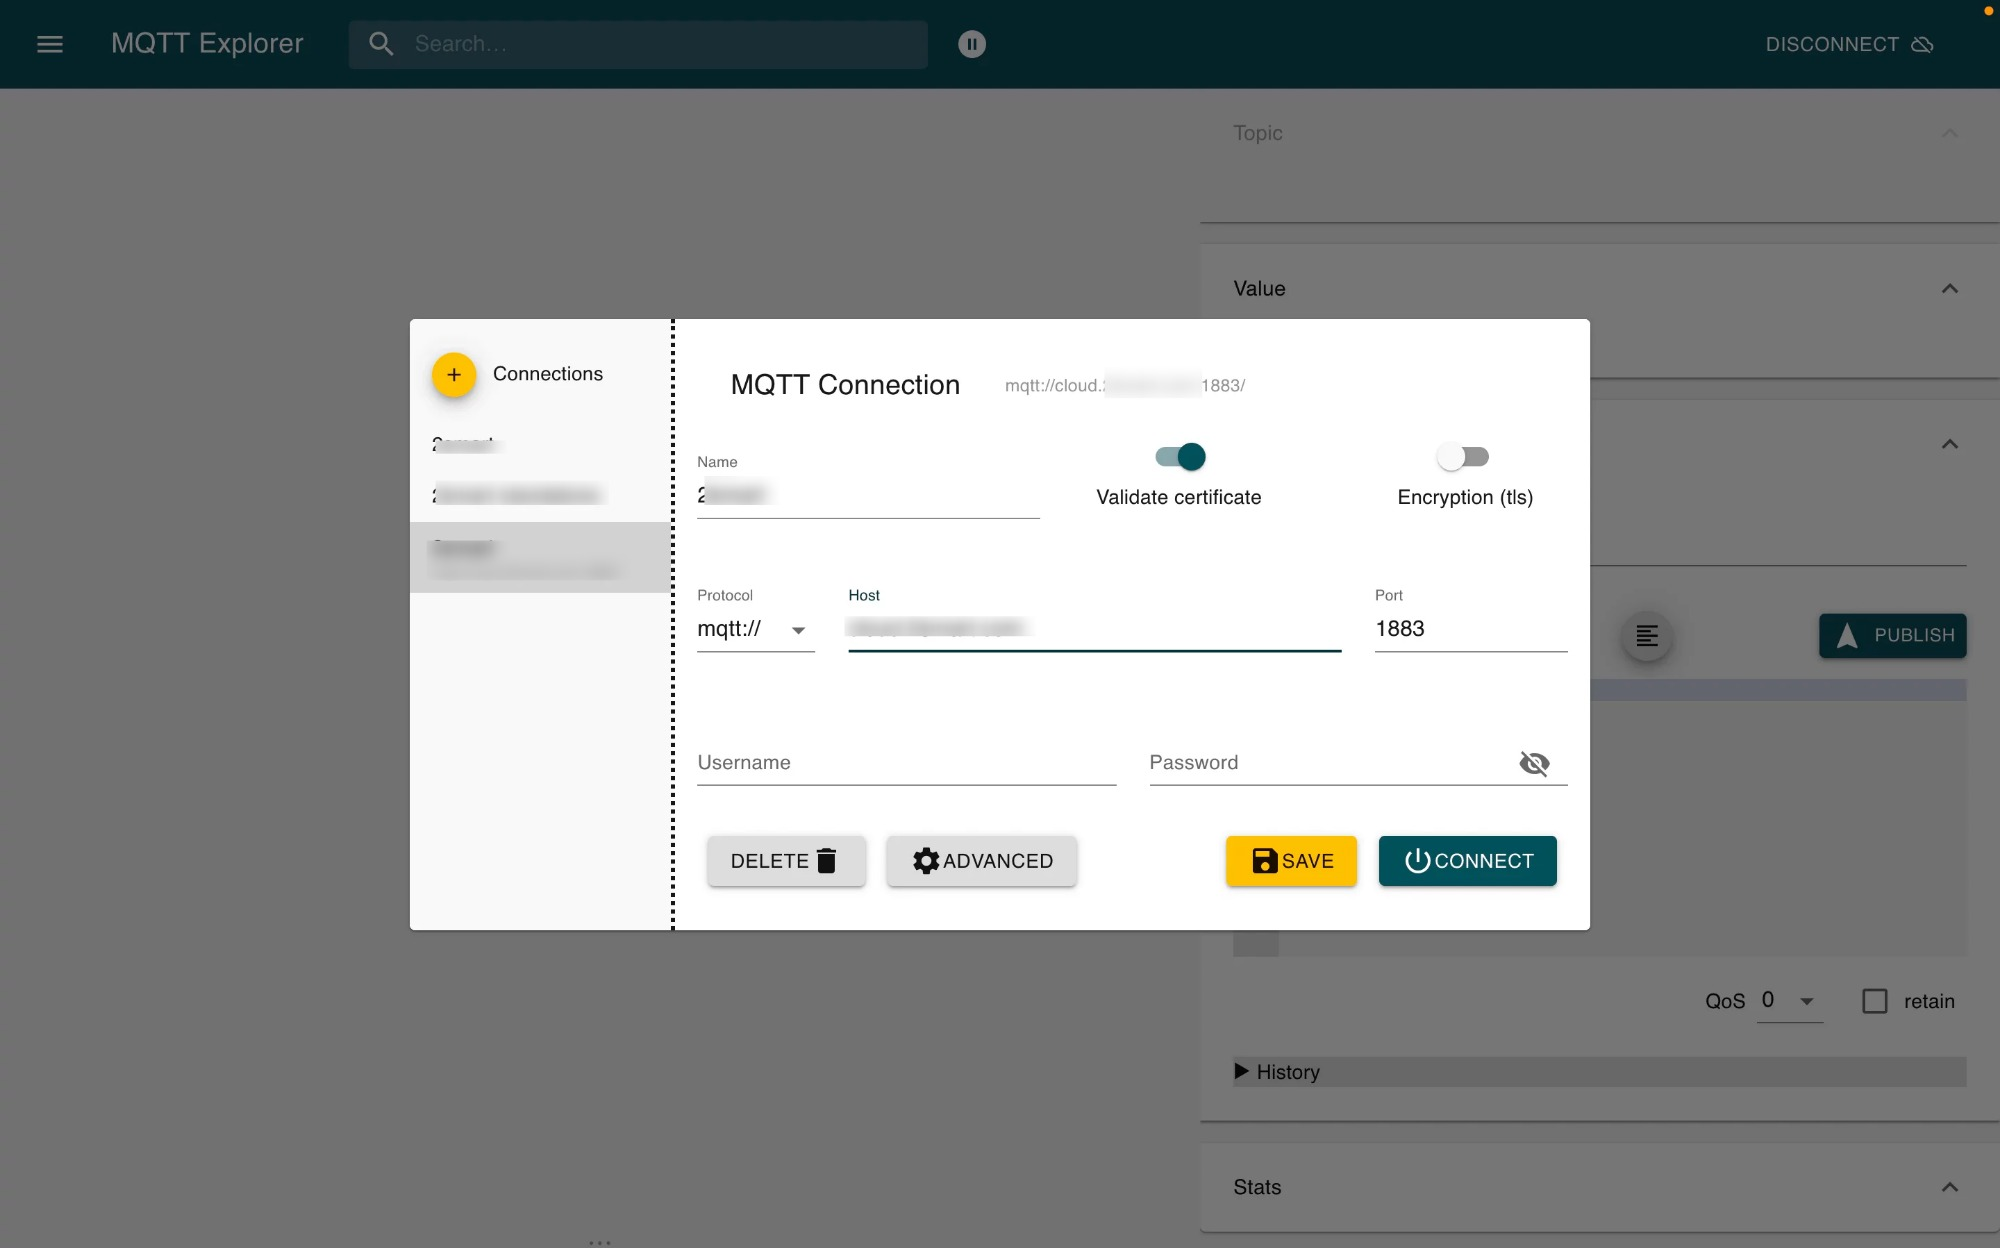
\includegraphics[width=1\textwidth]{chapters/3/img/15.jpg}
    \caption{cp 242-1 LEAN}
    \label{fig:campus}
\end{figure}
\begin{itemize}
    \item \textbf{Data Transmission}: Controllers publish sensor data to the MQTT broker, which is then consumed by backend services for processing.
    \item \textbf{Event-Based Architecture}: The platform reacts to changes instantly, ensuring timely updates and alerts.
\end{itemize}
\begin{figure}[H]
    \centering
    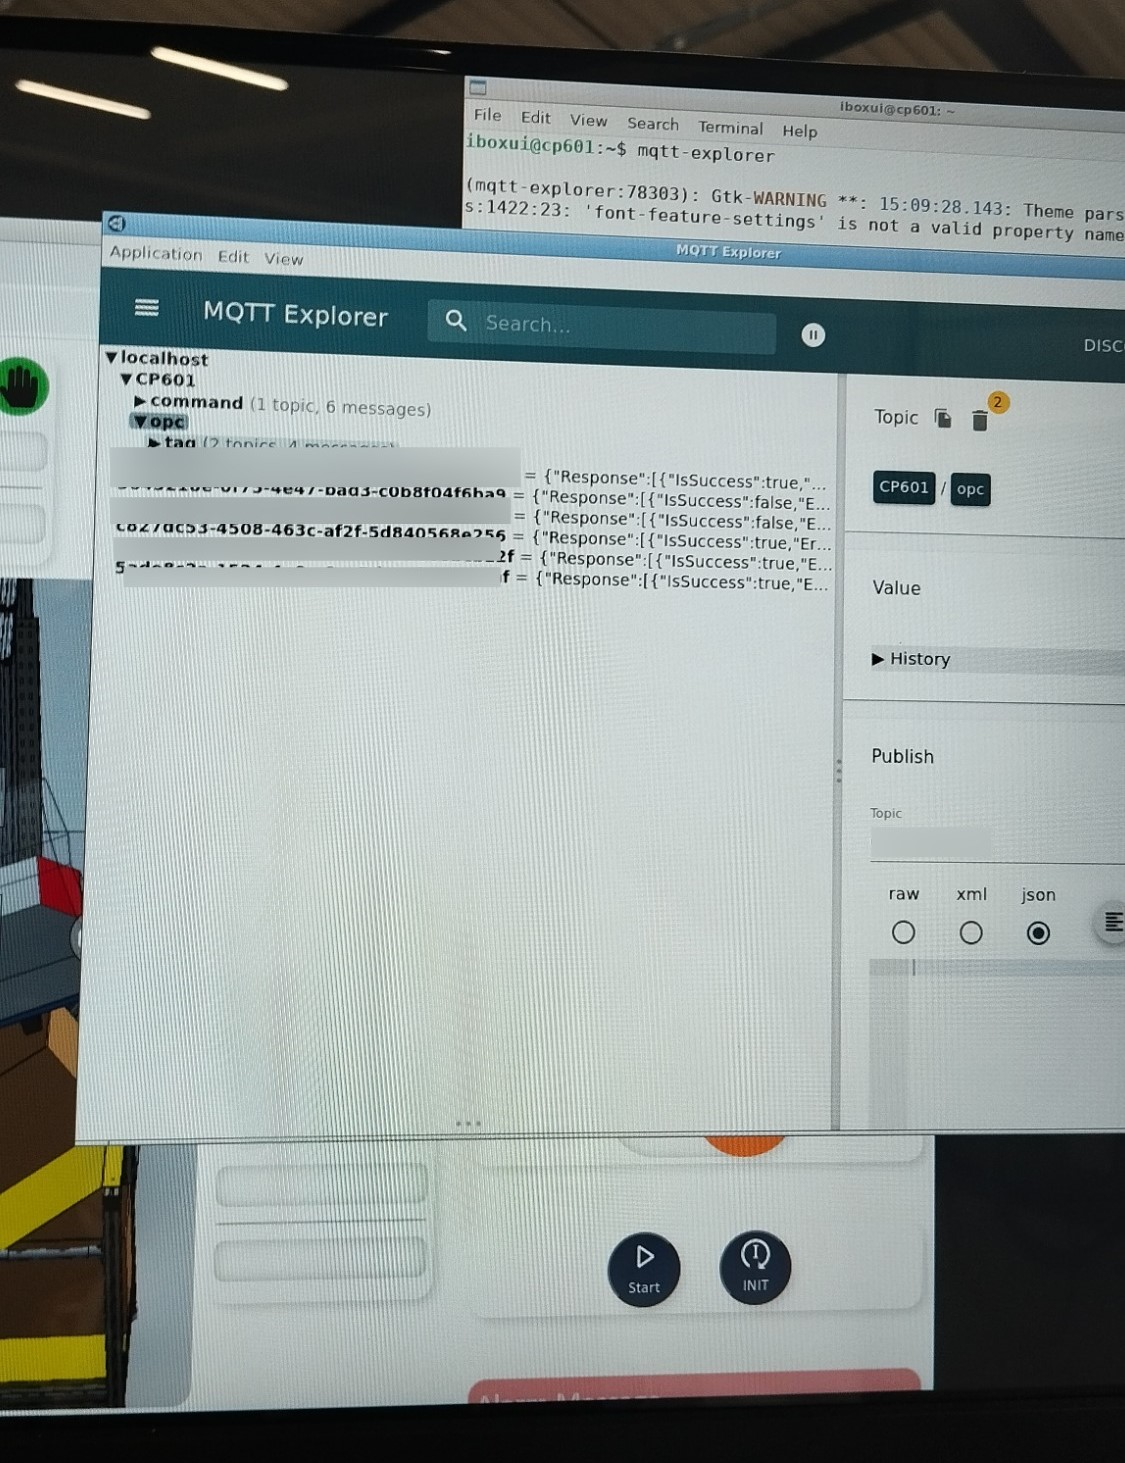
\includegraphics[width=0.6\textwidth]{chapters/3/img/14.jpg}
    \caption{cp 242-1 LEAN}
    \label{fig:campus}
\end{figure}


\subsection{Integration with Industrial Controllers (Step7 Siemens)}
The Siemens Step7 software was used to program controllers that manage laboratory equipment. The controllers were integrated with the LAB.E.S platform via MQTT, enabling automated data collection and control.
